\documentclass[a4paper]{article}

\usepackage[swedish]{babel}
\usepackage[utf8x]{inputenc}

\usepackage[vmargin=3cm,hmargin=2cm]{geometry}
\usepackage{parskip}
\usepackage[runin]{abstract}
\renewcommand{\abstitleskip}{0mm}

\usepackage{placeins}
\usepackage{hyperref}
\usepackage{amsmath}
\usepackage[T1]{fontenc}
\usepackage{graphicx}

\addto\extrasswedish{%
	\def\equationautorefname{Ekvation}%
	\def\figureautorefname{Figur}%
	\def\tableautorefname{Tabell}%
	\def\sectionautorefname{Rubrik}%
	\def\subsectionautorefname{Underrubrik}%
	\def\pageautorefname{Sida}%
}

% Hack för att få komma istället för punkt i matematiska uttryck
% $3.141592$ blir 3,141592
% Om man använder komma direkt får man ett litet oönskat mellanrum:
% $3,141592$ blir 3, 141592
\DeclareMathSymbol{,}{\mathpunct}{letters}{"3B}
\DeclareMathSymbol{.}{\mathord}{letters}{"3B}
\DeclareMathSymbol{\decimal}{\mathord}{letters}{"3A}

% Kommando för att få icke-kursiva enheter i matematiska uttryck
% $10\unit{km}$ blir 10 km
\newcommand{\unit}[1]{\ensuremath{\,\mathrm{#1}}}

\usepackage{lastpage}
\usepackage{fancyhdr}
\pagestyle{fancy}
\fancyhf[C]{\thepage}
\fancyhead[C]{Statik och Partikeldynamik, FMEA05}
\fancyhead[R,L]{}
\fancypagestyle{plain}{
  \fancyhead{}
}
\setcounter{secnumdepth}{-1}

\title{Fin titel}
\author{Anton Johansson\\Marcus Lindell Biehl\\Lunds Universitet}

\makeatletter

\renewcommand*\maketitle{
  {
    \begin{center}
      {\huge\bfseries \@title}\\
      \vspace{5mm}
      {\large \@author}
    \end{center}
    \vspace{2mm}
  }
}
\makeatother

\begin{document}
\maketitle

\begin{abstract}
  %Kort beskrivning  av resultaten (5-10  rader). Det ska inte  vara en
  %innehållsbeskrivning (först gör vi det, sen använder vi den metoden,
  %och så jämför vi det med de där tidigare kända resultaten, etc) utan
  %vara   koncentrerat  till   ”resultatet”,   vad   man  kommer   fram
  %till. Sammanfattningen är uppsatsens löpsedel. Den ska vara kort och
  %kärnfull och locka läsare genom att  effektivt göra klart vad det är
  %man uppnår genom att läsa rapporten.
\end{abstract}

\vspace{2mm}

\section{Inledning}

\subsection{Syfte}

\subsection{Ballistisk bana}

\subsection{Luftmotstånd}

\subsection{Corioliseffekten}

\section{Metod}

\section{Resultat}

\begin{figure}[h!]
	\centering
	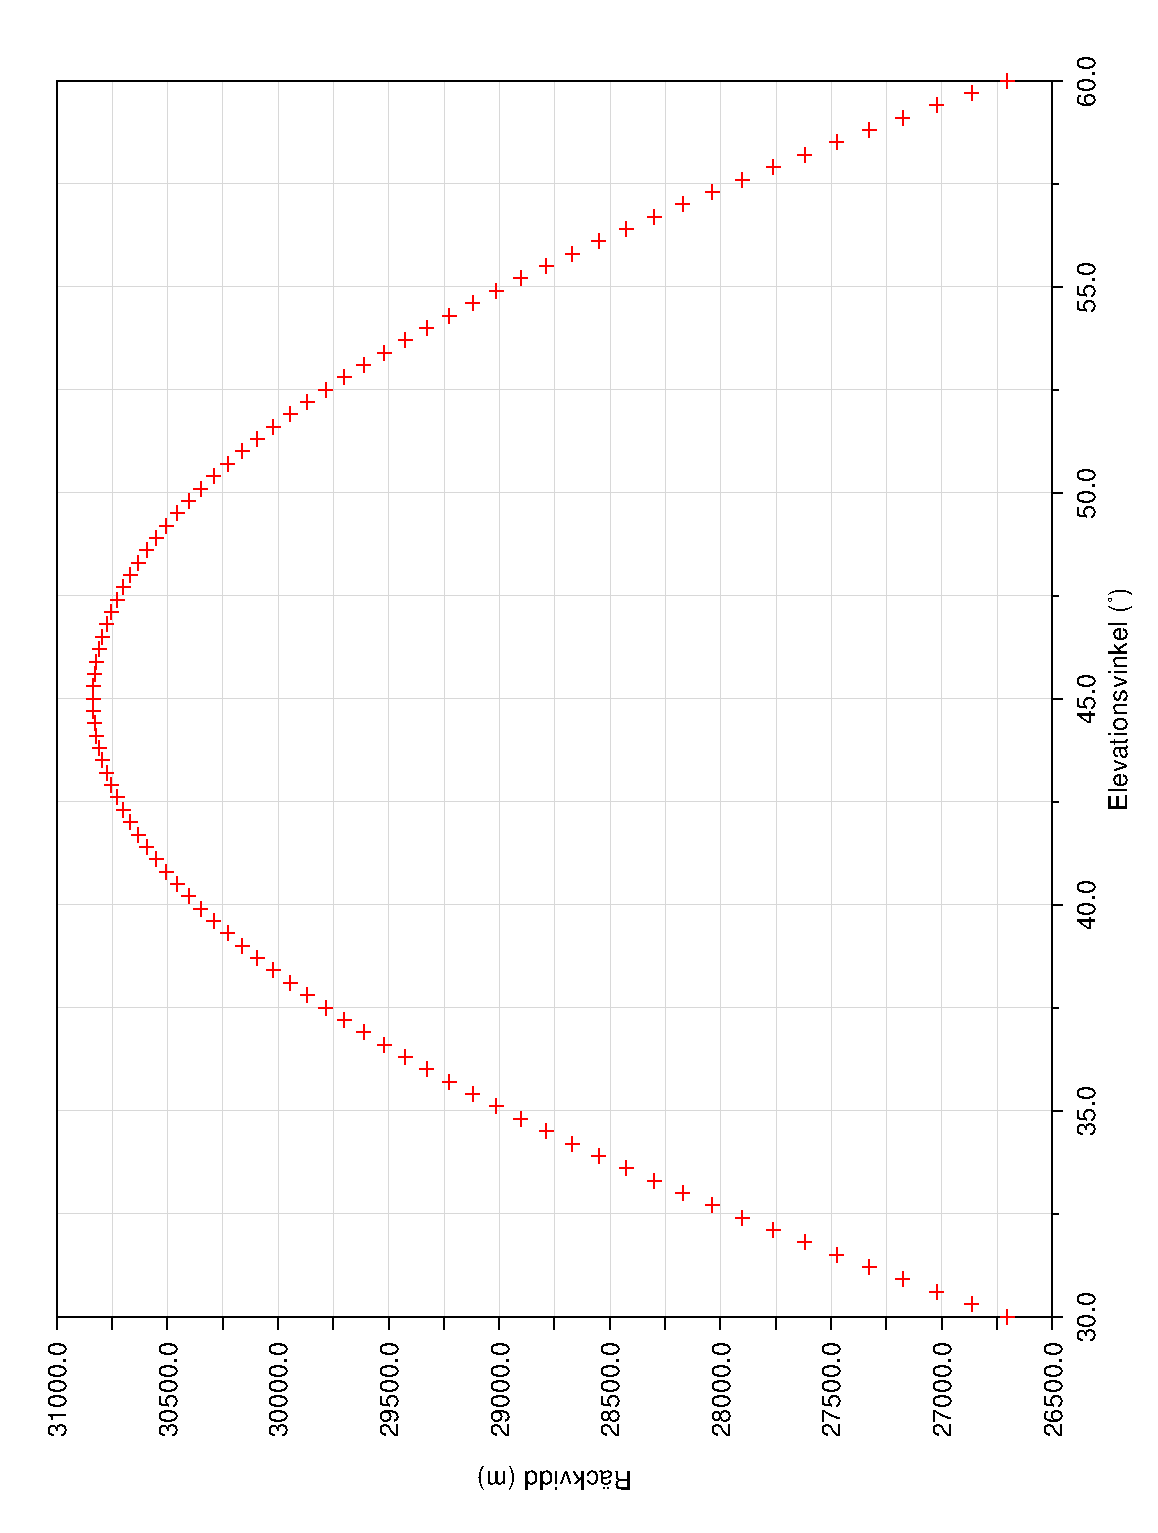
\includegraphics[width=0.5\linewidth, angle=-90]{Data/ProjektilH0.eps}
	\caption{Räckvidd som funktion av elevationsvinkel med $H = 0$. Utan luftmotstånd/Corioliseffekt}
	\label{fig:projektilH0}
\end{figure}

\begin{figure}[h!]
	\centering
	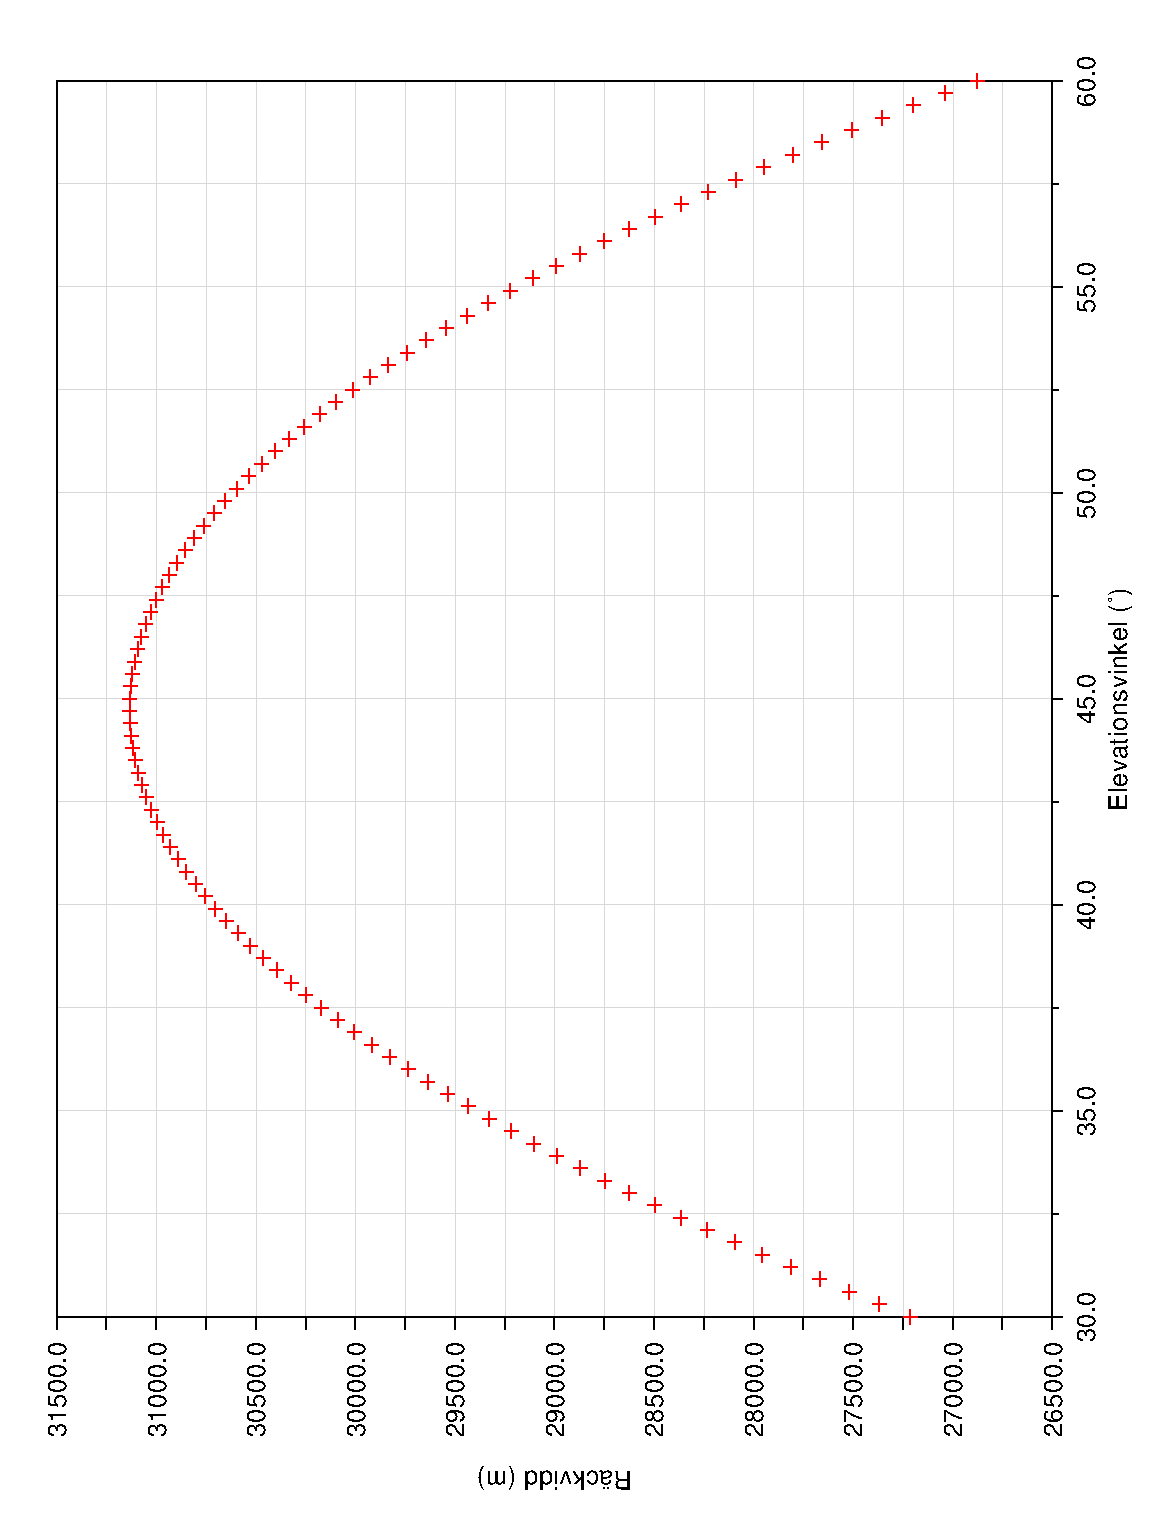
\includegraphics[width=0.5\linewidth, angle=-90]{Data/ProjektilH300.eps}
	\caption{Räckvidd som funktion av elevationsvinkel med $H = 300$. Utan luftmotstånd/Corioliseffekt}
	\label{fig:projektilH300}
\end{figure}

\begin{figure}[h!]
	\centering
	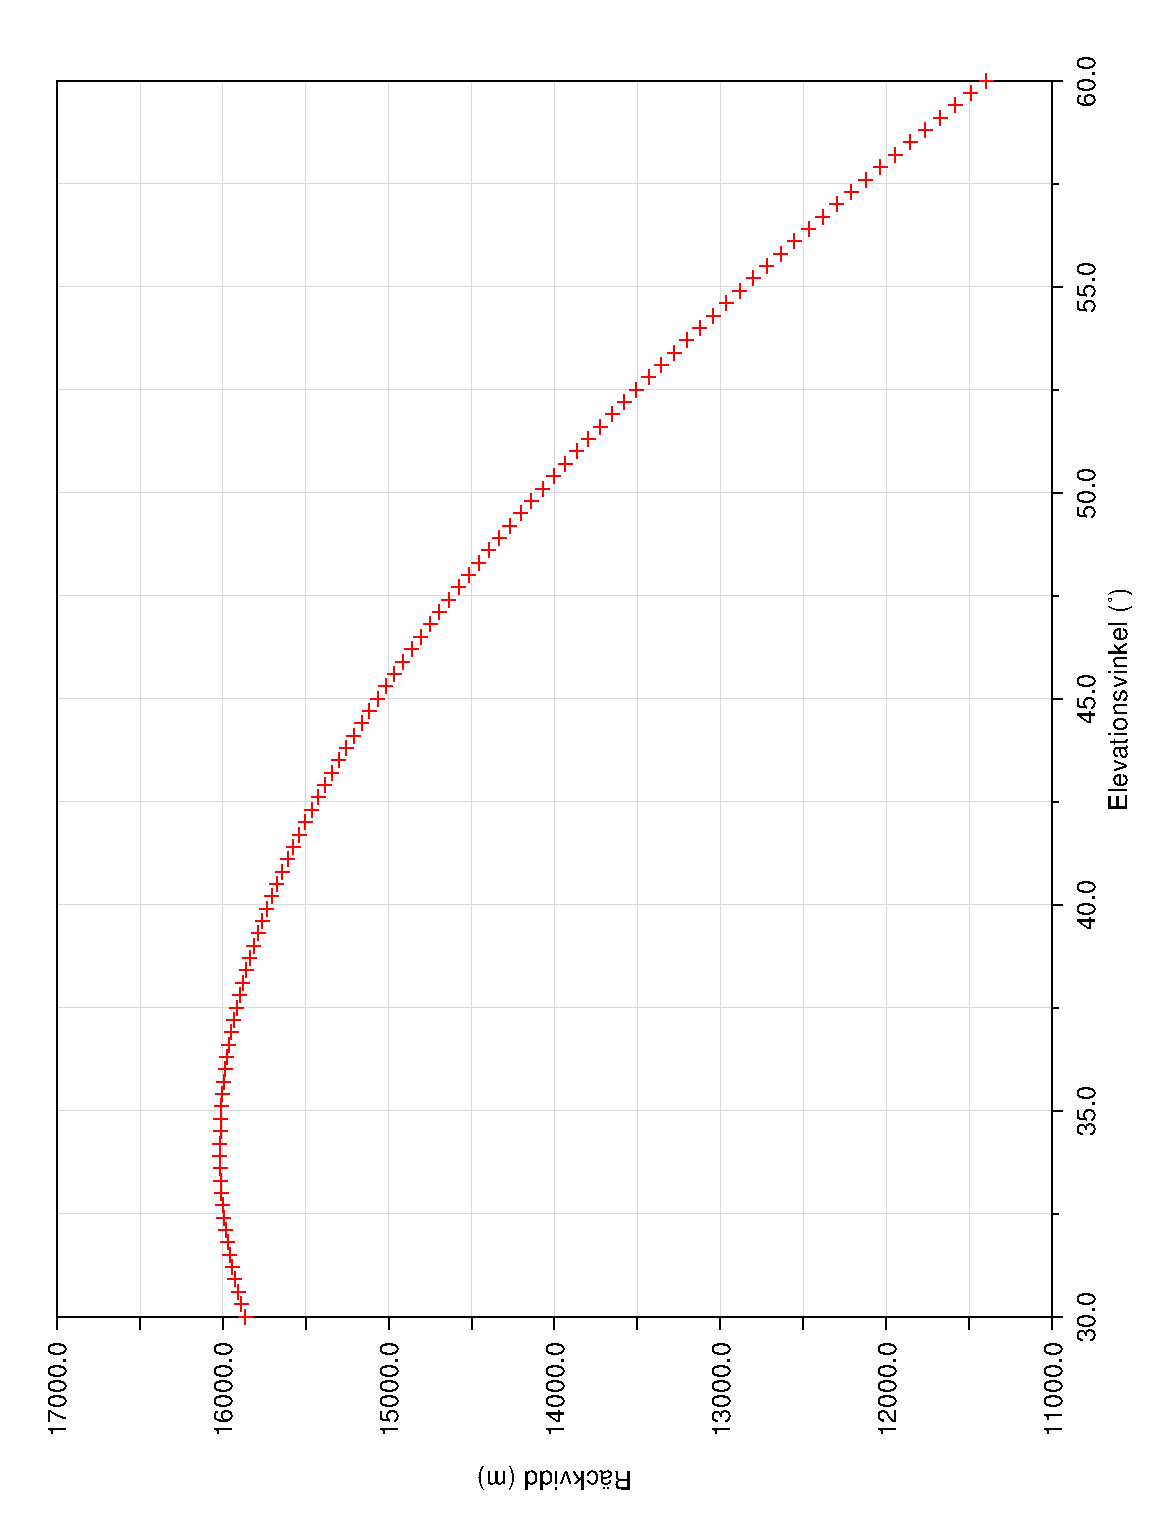
\includegraphics[width=0.5\linewidth, angle=-90]{Data/ProjektilH300Drag.eps}
	\caption{Räckvidd som funktion av elevationsvinkel med $H = 300$. Med luftmotstånd, utan Corioliseffekten}
	\label{fig:projektilH300Drag}
\end{figure}

\begin{figure}[h!]
	\centering
	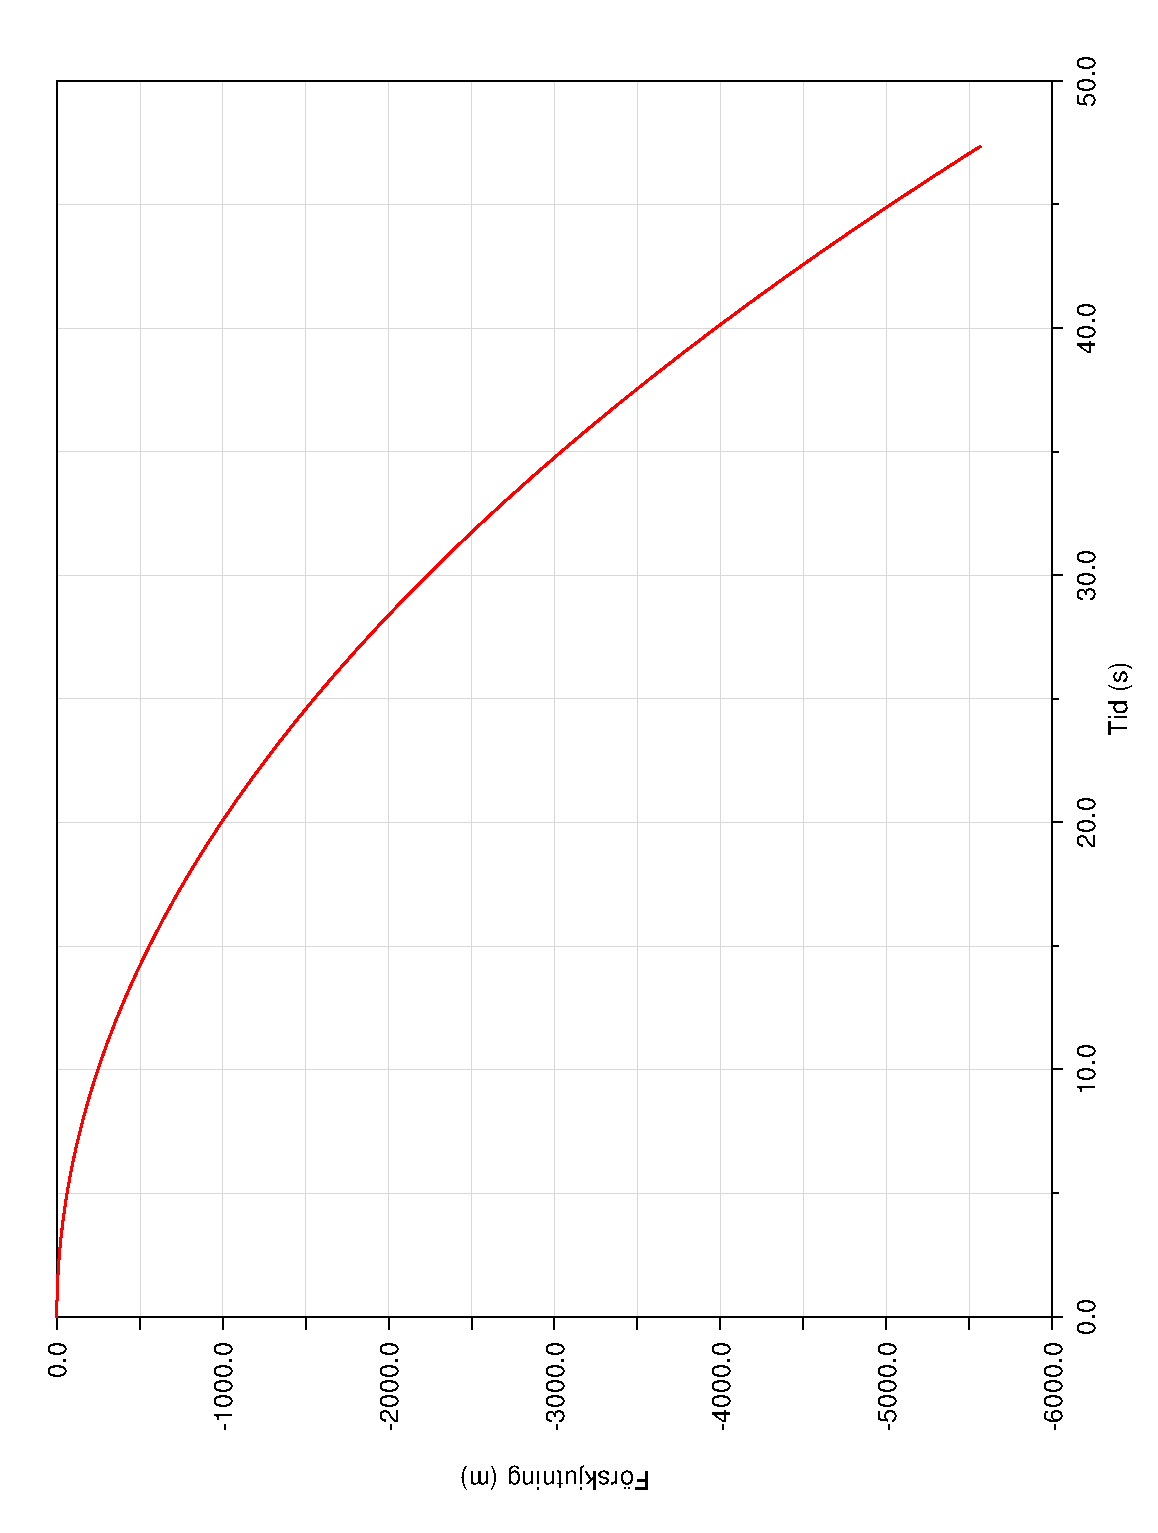
\includegraphics[width=0.5\linewidth, angle=-90]{Data/ZdisplacementAlpha0.eps}
	\caption{Förskjutning i z-led som funktion av tiden med $H = 300, \alpha = 0$. Med luftmotstånd och Corioliseffekten}
	\label{fig:ZAlpha0}
\end{figure}

\begin{figure}[h!]
	\centering
	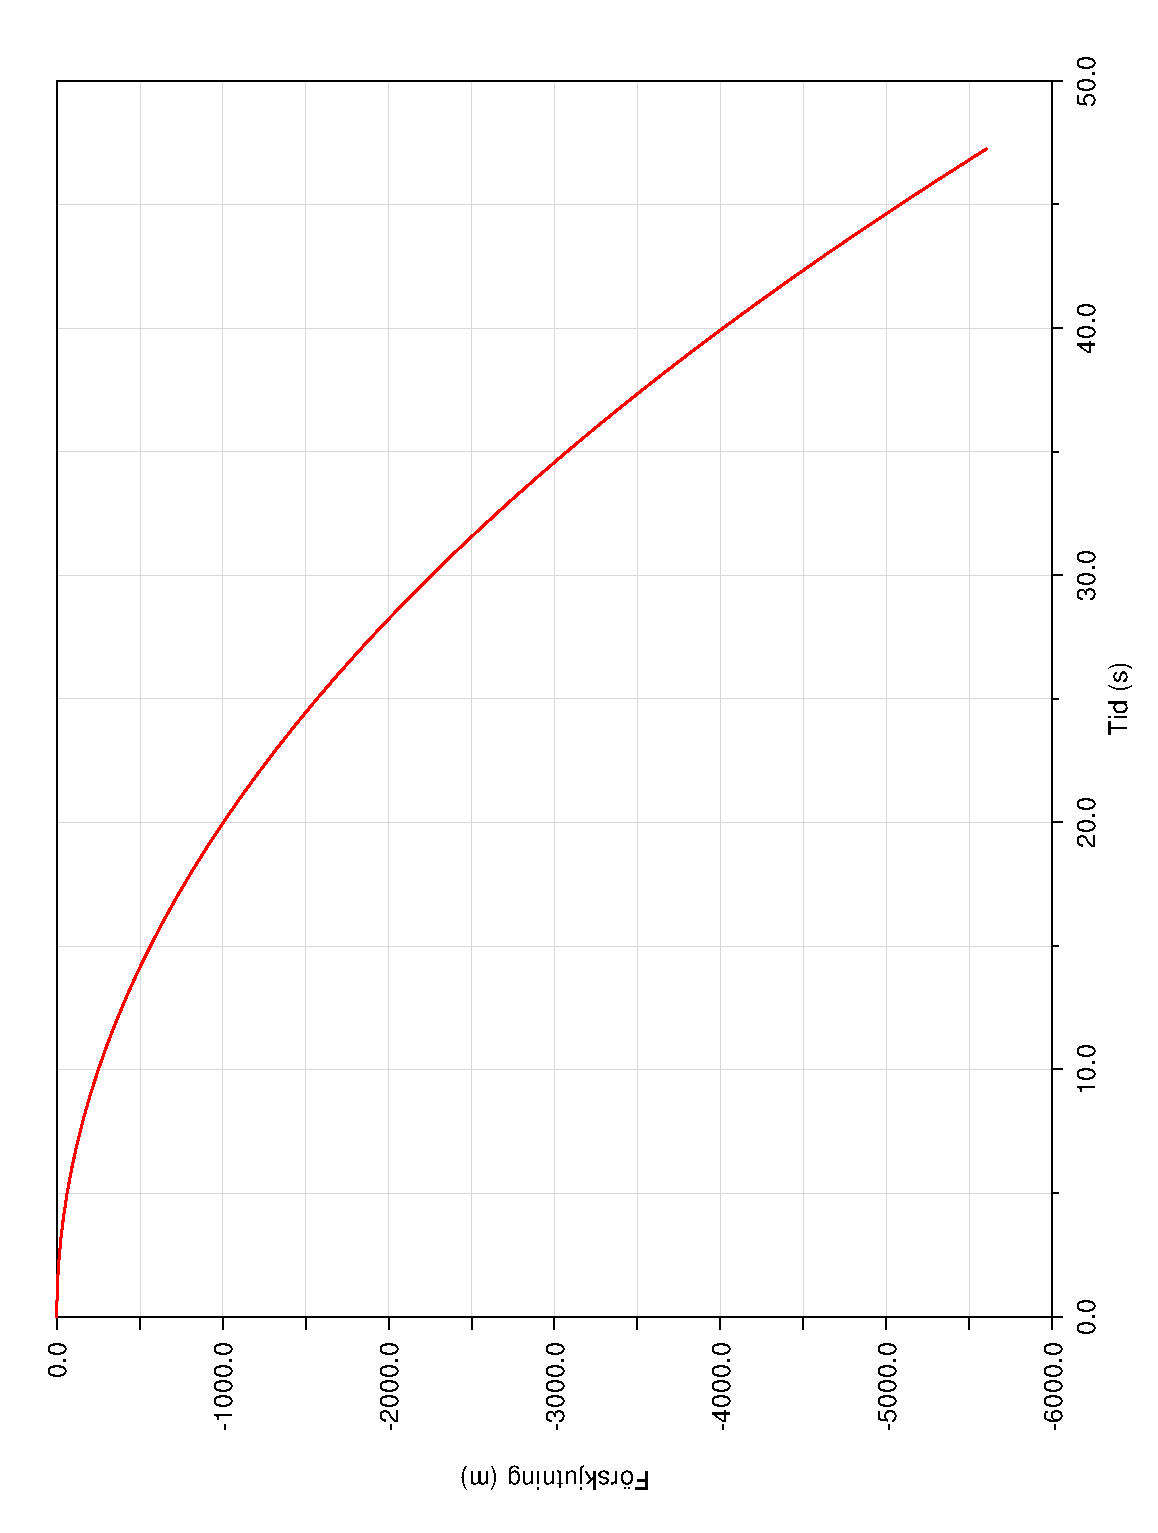
\includegraphics[width=0.5\linewidth, angle=-90]{Data/ZdisplacementAlpha0Lambda0.eps}
	\caption{Förskjutning i z-led som funktion av tiden med $H = 300, \alpha = 0, \lambda = 0$. Med luftmotstånd och Corioliseffekten}
	\label{fig:ZAlpha0Lambda0}
\end{figure}

\begin{figure}[h!]
	\centering
	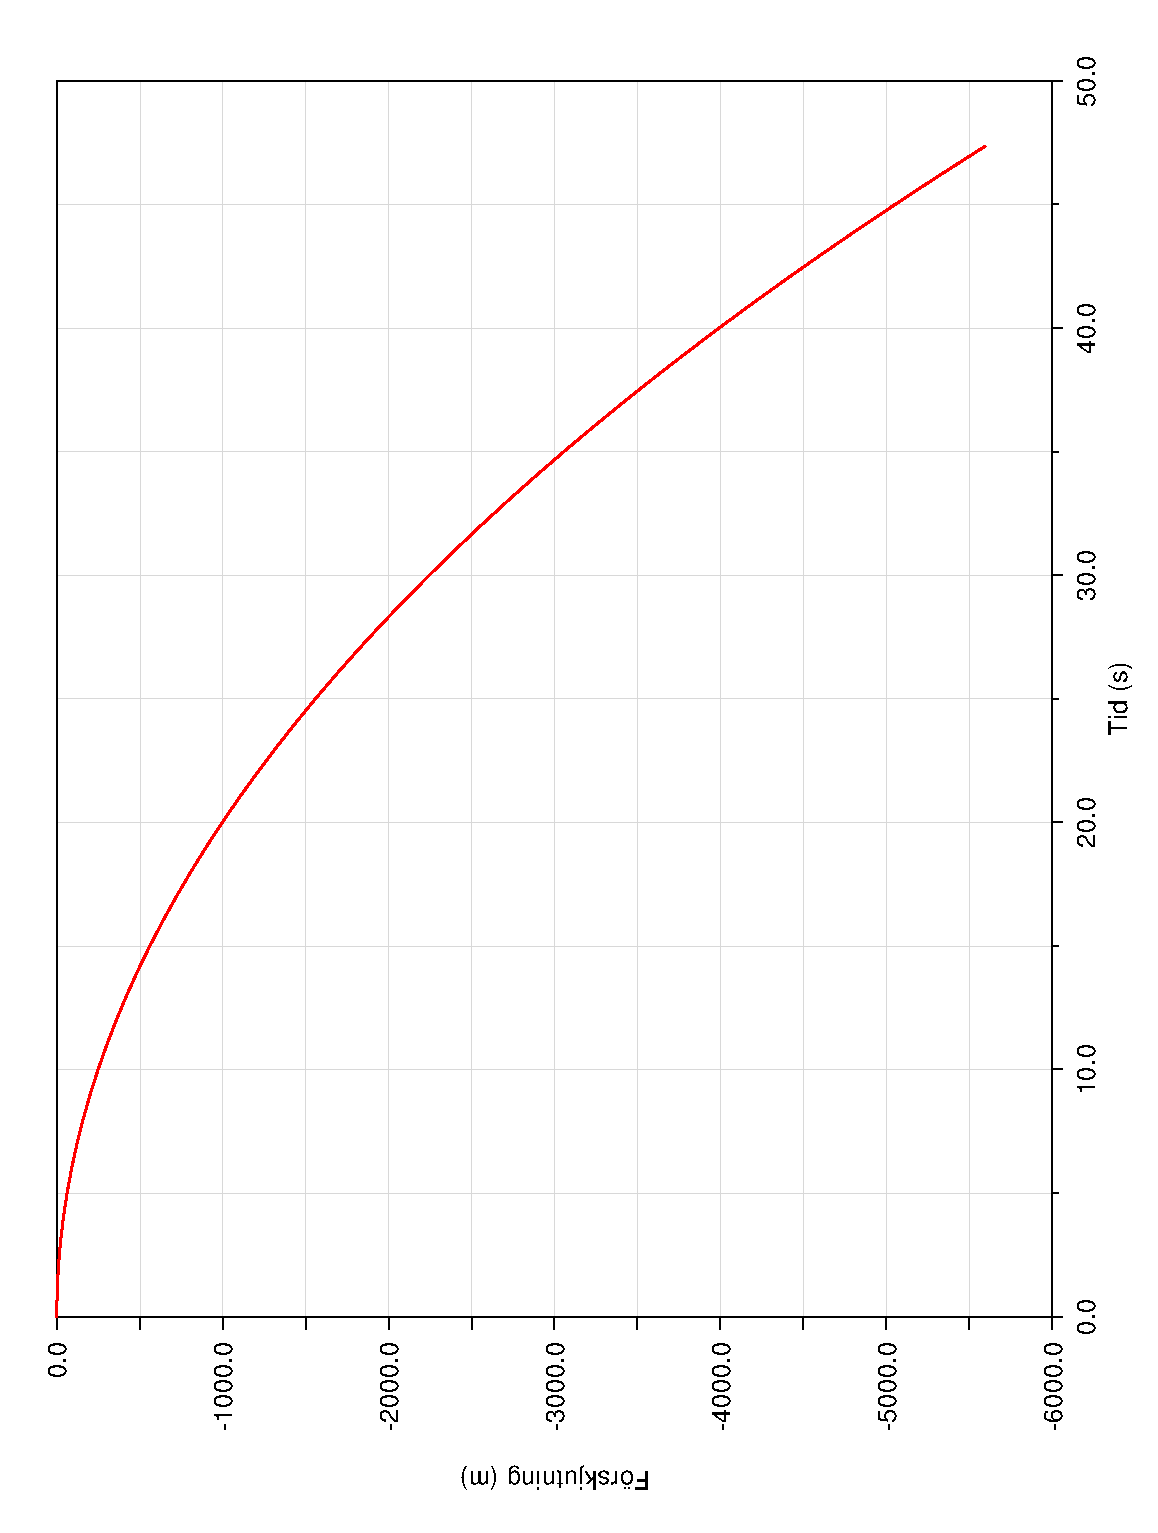
\includegraphics[width=0.5\linewidth, angle=-90]{Data/ZdisplacementAlpha90.eps}
	\caption{Förskjutning i z-led som funktion av tiden med $H = 300, \alpha = 90$. Med luftmotstånd och Corioliseffekten}
	\label{fig:ZAlpha90}
\end{figure}

\begin{figure}[h!]
	\centering
	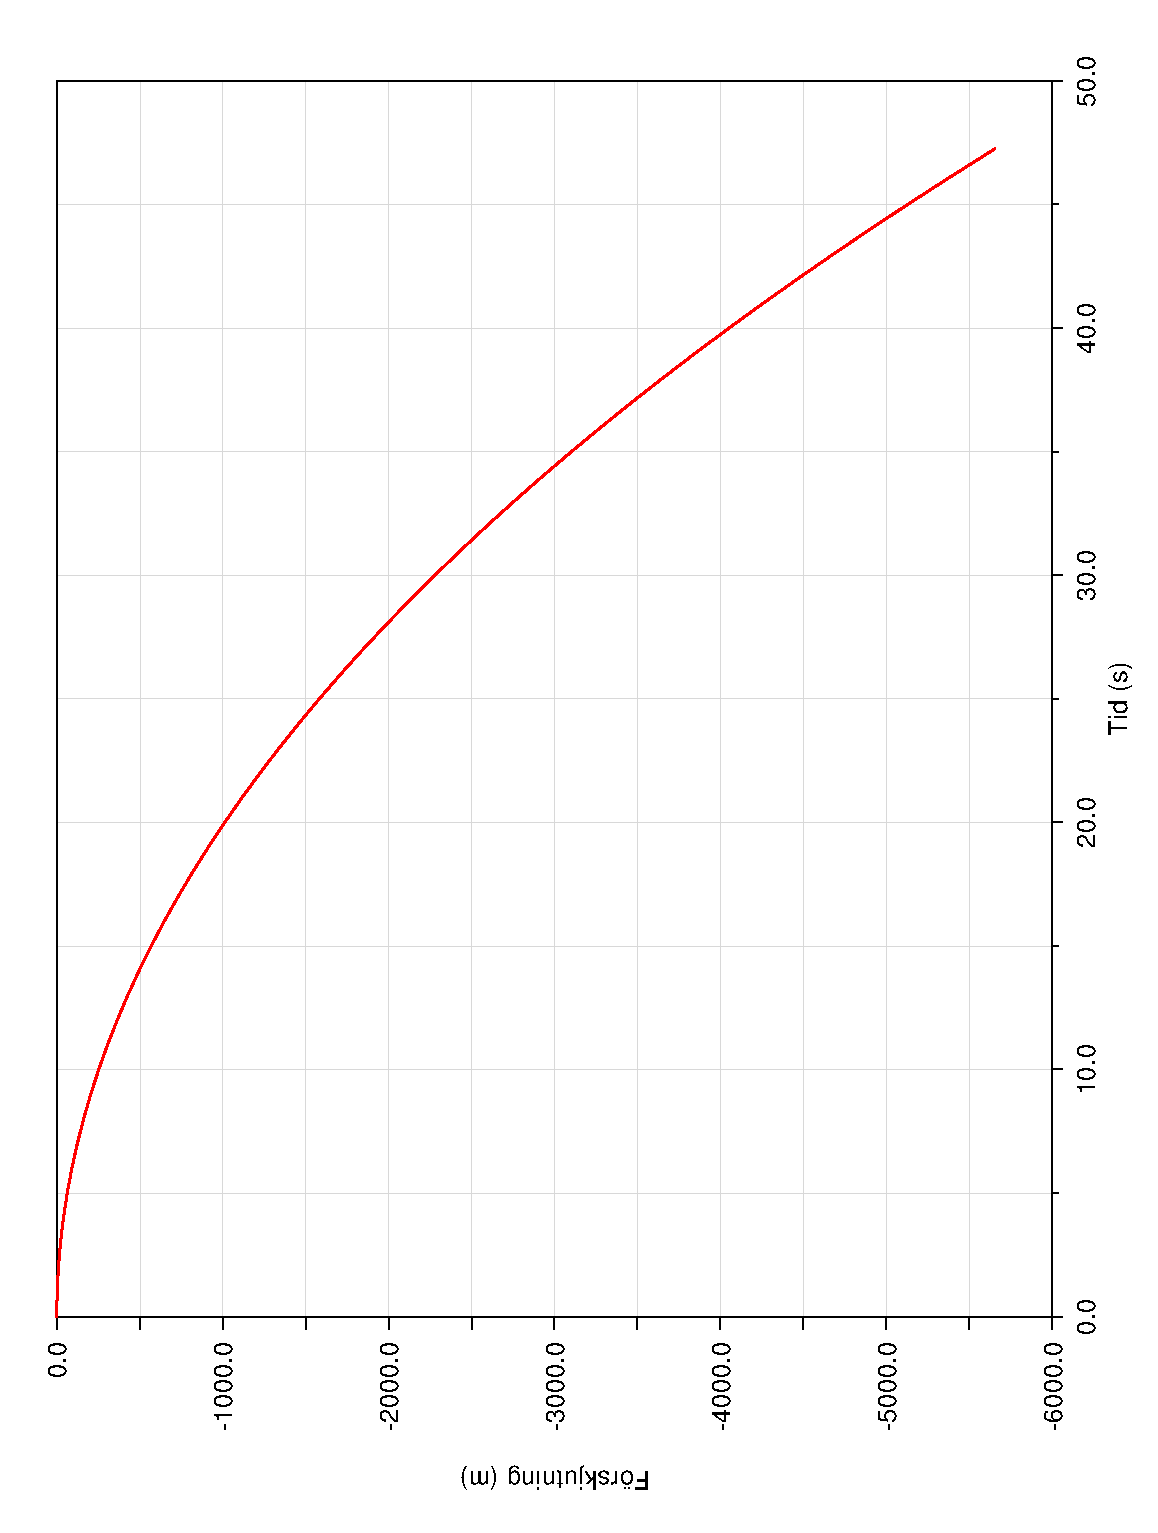
\includegraphics[width=0.5\linewidth, angle=-90]{Data/ZdisplacementAlpha90Lambda0.eps}
	\caption{Förskjutning i z-led som funktion av tiden med $H = 300, \alpha = 90, \lambda = 0$. Med luftmotstånd och Corioliseffekten}
	\label{fig:ZAlpha90Lambda0}
\end{figure}

\section{Diskussion}

\section{Slutsats}

\end{document}

